%%% Local Variables:
%%% mode: LaTeX
%%% TeX-master: t
%%% End:
%%% TeX-command-extra-options: "-shell-escape"

\documentclass{beamer}
\usetheme{Madrid}
\usepackage{palatino}
\usepackage{tikz}
\usepackage{graphicx}
\usepackage{svg}

\usepackage[T1]{fontenc}
\usepackage[utf8]{inputenc}
\usefonttheme[onlymath]{serif}



\date[]{}
\title[La recherche du meilleur coup.]{À la recherche du meilleur coup au jeu d'Awalé}
\author[Nils Lelorieux]{Nils Lelorieux}
\institute[]{numéro de candidat : 24296}

\begin{document}

\begin{frame}
  \titlepage
\end{frame}
 
\begin{frame}
  \frametitle{Introduction}

  \begin{minipage}[b]{0.3\linewidth}
    \begin{figure}
      \centering
      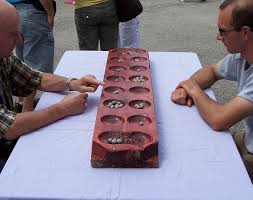
\includegraphics[width=1.1\linewidth]{ressources/photo_joueur_awale.jpeg}
      \caption{Une partie d'Awalé}
      \label{fig:mon_image}
    \end{figure}
  \end{minipage}
  \hfill
  \begin{minipage}[b]{0.3\linewidth}
    \begin{figure}
      \centering
      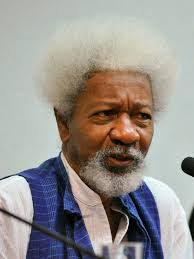
\includegraphics[width=0.7\linewidth]{ressources/wole_soyinka.jpeg}
      \caption{Photographie de Wole Soyinka}
      \label{fig1}
    \end{figure}
  \end{minipage}
  \hfill
  \begin{minipage}[b]{0.3\linewidth}
    \begin{figure}
      \centering
      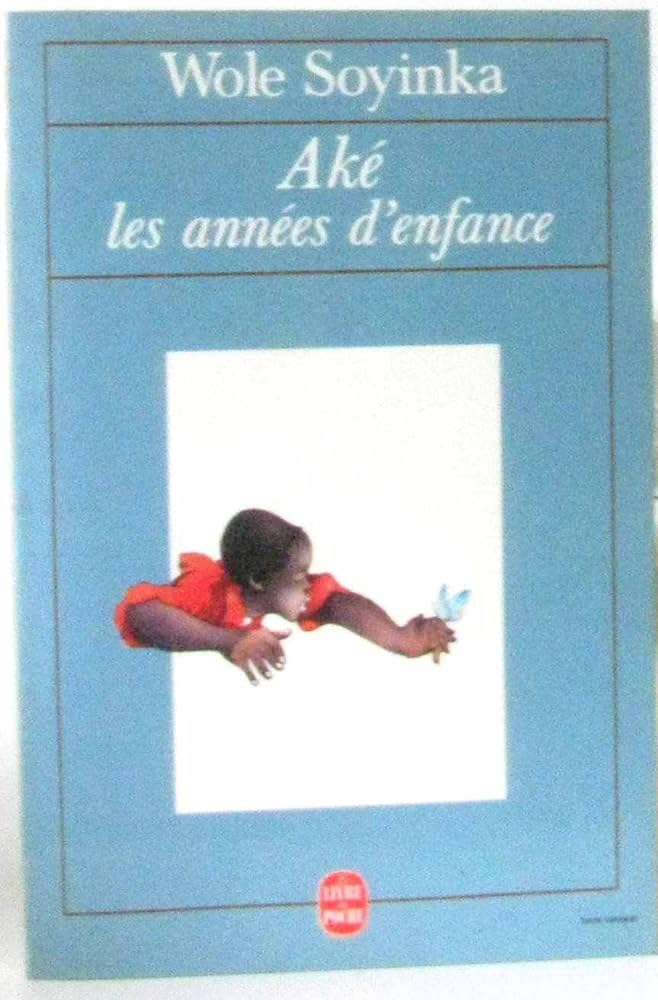
\includegraphics[width=0.9\linewidth]{ressources/ake_les_annees_denfance.png}
      \caption{Couverture du livre "Aké les années d'enfance"}
      \label{fig2}
    \end{figure}
  \end{minipage}

\end{frame}


\begin{frame}
  \frametitle{Un jeu ancien et important}
  \begin{figure}
    \centering
    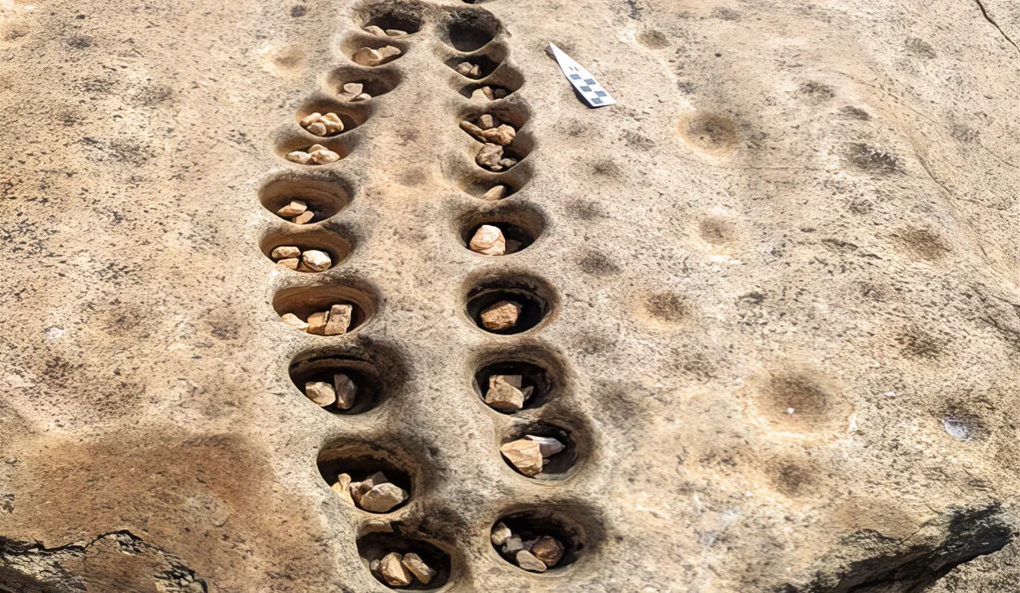
\includegraphics[width=\linewidth]{ressources/ancien_plateau_jeu.png}
    \caption{Un ancien plateau de jeu découvert au Kenya}
  \end{figure}
\end{frame}


\begin{frame}
  \begin{block}{Problématique}
    L'étude théorique du jeu d'Awalé permet-elle de toujours jouer le meilleur coup, ou l'utilisation d'algorithmes est-elle indispensable ?
  \end{block}
  \frametitle{Vue d'ensemble}
  \tableofcontents
\end{frame}


\section{Présentation des règles du jeu et motivations}

\begin{frame}
  \frametitle{Déroulé d'une partie (1)}
  \begin{figure}
    \centering
    \includesvg[width=0.5\linewidth]{ressources/diagramme_debut_partie.svg}
    \caption{2 coups joués par les 2 joueurs en début de partie}
  \end{figure}
\end{frame}

\begin{frame}
  \frametitle{Déroulé d'une partie (2)}
  \begin{figure}
    \centering
    \includesvg[width=1\linewidth]{ressources/diagramme_capture.svg}
    \caption{Position où le joueur Sud capture les pierres du joueur Nord}
  \end{figure}
\end{frame}

\begin{frame}
  \frametitle{Règles du jeu}
  \begin{itemize}
  \item<Règles du jeu>
  \item Deux joueurs s'affrontent.
  \item 4 graines dans les 12 trous divisés en deux rangées de six.
  \item Le premier joueur choisi un puit et sème les graines.
  \item Si le dernier puit semé contient 2 ou 3 pierres, il les récupère et fait la même chose dans le puit précédent, ...
  \item Le gagnant est le joueur qui a le plus de pierres
  \end{itemize}
\end{frame}

\begin{frame}
  \frametitle{Motivations}
  \begin{block}{Motivation}
    Pourquoi avoir choisi d'étudier le jeu d'Awalé ?
  \end{block}
  
  \begin{itemize}
  \item C'est un jeu important.
  \item Le facteur d'embrachement est faible.
  \item Possibilité d'utiliser des algorithmes classiques de la théorie des jeux pour trouver le coup optimal
  \item Il y a $279 \ 871 \ 768 \ 995 $ états possibles ($2\times 10^{20}$ pour le puissance 4, un jeu résolu).
  \end{itemize}
\end{frame}

\section{Échec de l'approche théorique et des premiers algorithmes}
\begin{frame}
  \frametitle{Une approche théorique}
  \begin{itemize}
  \item Étude des positions déterminées : une position où Sud capture à tous les coups et laisse une seule pierre à Nord.
  \item Correspondance avec un autre jeu de Mancala : le jeu de Tchoukaillon \footnote{B.Jones, L.Taalman, A.Tongen : Solitaire Mancala Games and the Chinese Remainder Theorem}
  \item Il existe une périodicité sur le nombre de pierre dans une position déterminée : inutile pour notre étude. \footnote{D.Broline, D.Loeb : The Combinatorics of Mancala-type games: Ayo, Tchoukaillon, and $\frac 1 \pi$}
  \item Il n'existe que 48 positions déterminées (le nombre de pierres).
  \end{itemize}
\end{frame}

\begin{frame}
  \frametitle{L'algorithme min-max}
  \begin{figure}
    \centering
    \includesvg[width=1\linewidth]{ressources/diagramme_min_max.svg}
    \caption{Déroulé min max au jeu de l'Awalé }
  \end{figure}
\end{frame}


\begin{frame}
  \frametitle{Problème du min-max classique}
  \begin{figure}
    \centering
    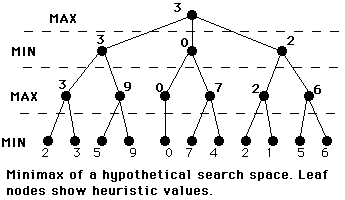
\includegraphics[width=0.8\linewidth]{ressources/min_max_heuristique.png}
    \caption{Un exemple de min max avec heuristique}
  \end{figure}
\end{frame}

\begin{frame}
  \frametitle{Résultat min-max}
  \begin{figure}
    \centering
    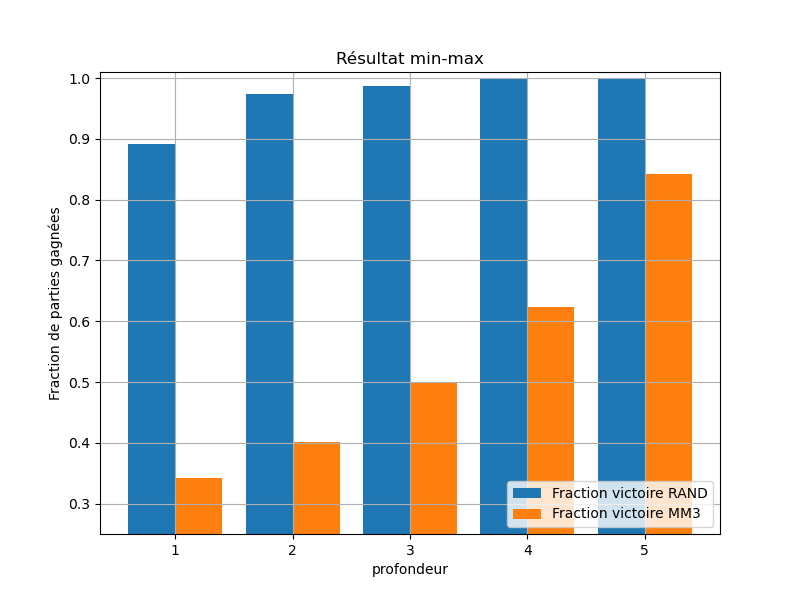
\includegraphics[width=0.75\linewidth]{ressources/resultat_min_max.png}
    \caption{Résultats de l'algorithme min-max (1000 parties)}
  \end{figure}
\end{frame}

\begin{frame}
  \frametitle{Un algorithme de Monte Carlo}
  \begin{figure}
    \centering
    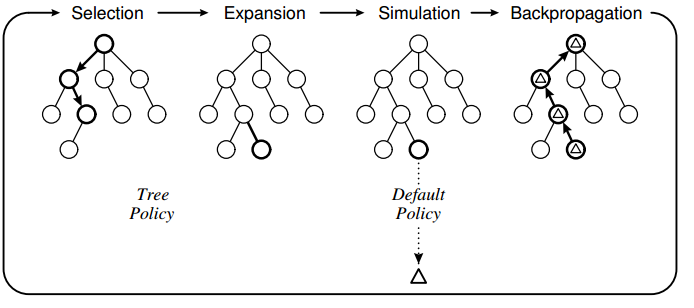
\includegraphics[width=\linewidth]{ressources/monte_carlo_explication.png}
    \caption{Principe de l'algorithme de Monte Carlo}
  \end{figure}
\end{frame}

\begin{frame}
  \frametitle{Des résultats peu convaincants}
  \begin{figure}
    \centering
    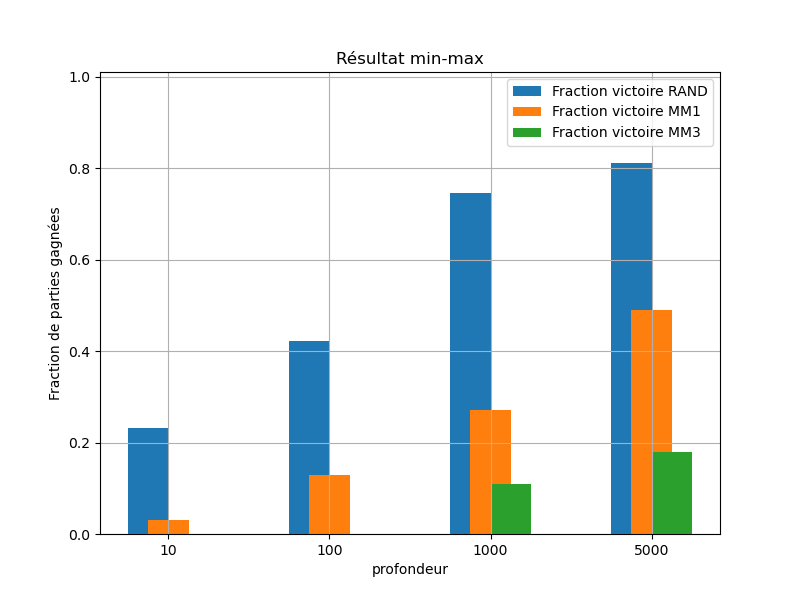
\includegraphics[width=0.75\linewidth]{ressources/resultat_flat_monte_carlo.png}
    \caption{Résultat de l'algorithme flat Monte Carlo (1000 parties)}
  \end{figure}
\end{frame}

\section{Des résultats concluents grâce à deux nouvelles techniques : la recherche arborescente de Monte-Carlo et l'analyse rétrograde}
\begin{frame}
  \frametitle{Une amélioration de l'algorithme précédent}
  \begin{figure}
    \centering
    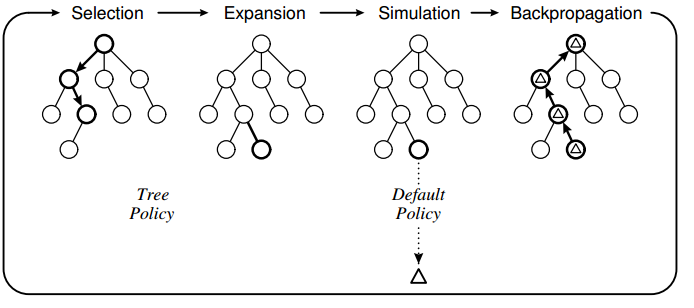
\includegraphics[width=\linewidth]{ressources/monte_carlo_explication.png}
    \caption{Principe de la recherche arborescente de Monte Carlo}
  \end{figure}
\end{frame}

\begin{frame}
  \frametitle{Comment choisir le noeud à explorer ?}
  \begin{block}{Score d'un noeud}
On attribue à chaque noeud $n$ un score $Q$ qui correspond à la moyenne des gains remportés part toutes les parties contenant le noeud $n$. Étant donné un noeud $n$ et son père $p$, on a :
$$ Q(n) = \frac 1 {N(n)} \sum_{i=1}^{N(p)}\mathbb I_i(n)z_i $$
où $N(n)$ représente le nombre de visites du noeud $n$, $z_i$ est le gain lors de la ième visite de noeud $n$ et $\mathbb I_i(n)$ vaut $1$ si le noeud $n$ a ete choisie à la $i$ visite par $p$, 0 sinon
  \end{block}
\end{frame}

\begin{frame}
  \frametitle{Comment choisir le noeud à explorer (2) ?}
  \begin{block}{Meilleur fils d'un noeud $n$}
    $$\underset{n' \in \text{ enfants de } n}{\arg\max} \frac {Q(n')} {N(n')} + c\sqrt{\frac {2ln(N(n))} {N(n')} }$$
  \end{block}
\end{frame}


\begin{frame}
  \frametitle{Visualisation des arbres}
   \begin{figure}
     \centering
     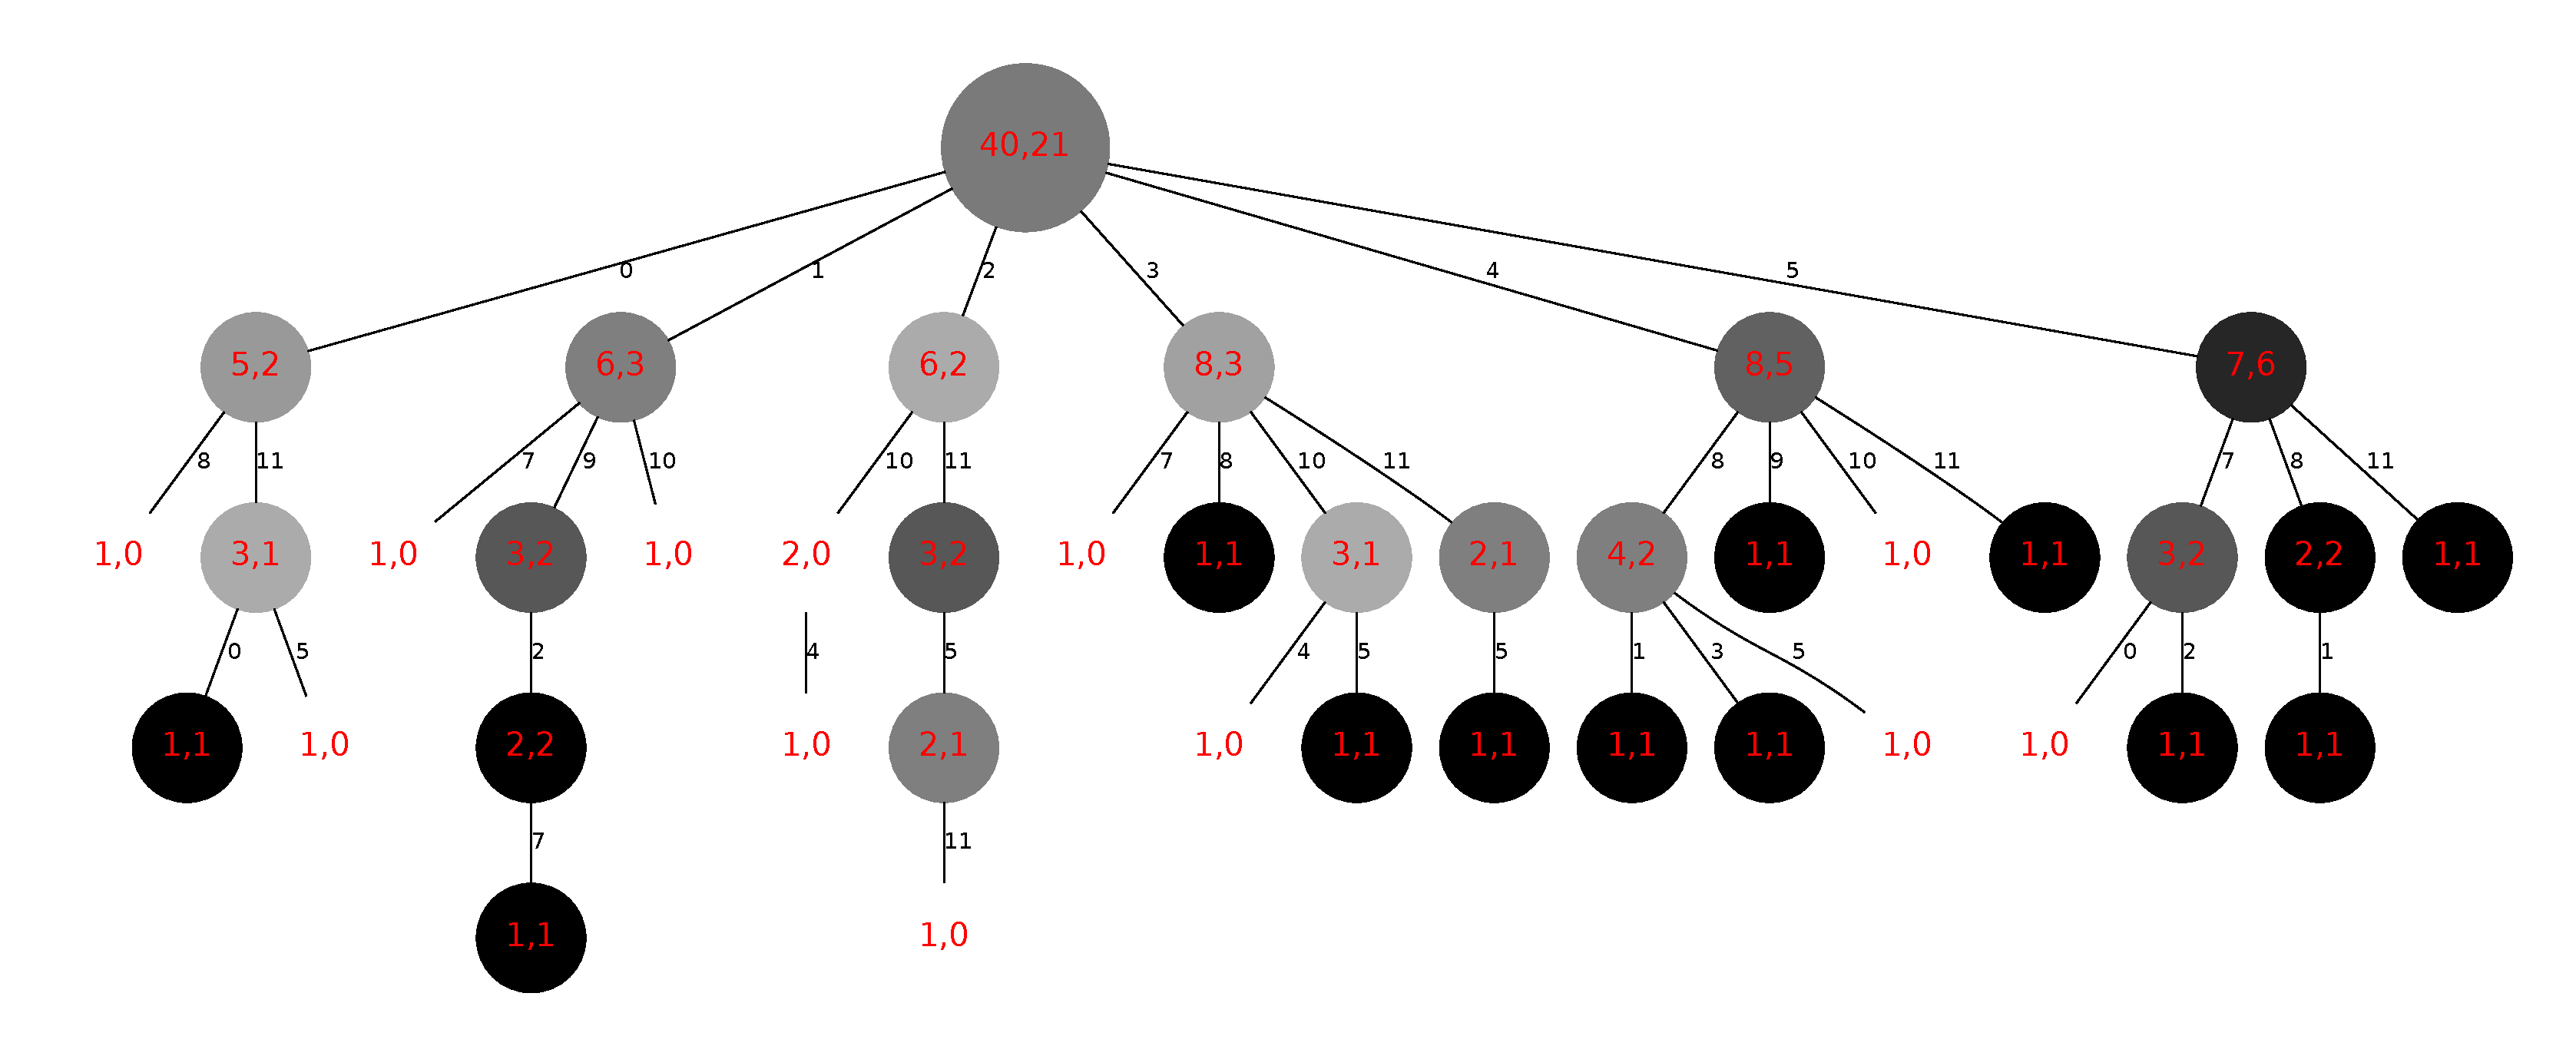
\includegraphics[width=\linewidth]{ressources/arbre_40_flat.pdf}
     \caption{Un arbre de recherche pour le flat Monte Carlo}
   \end{figure}
\end{frame}

\begin{frame}
  \frametitle{Visualisation des arbres}
  \begin{figure}
    \centering
    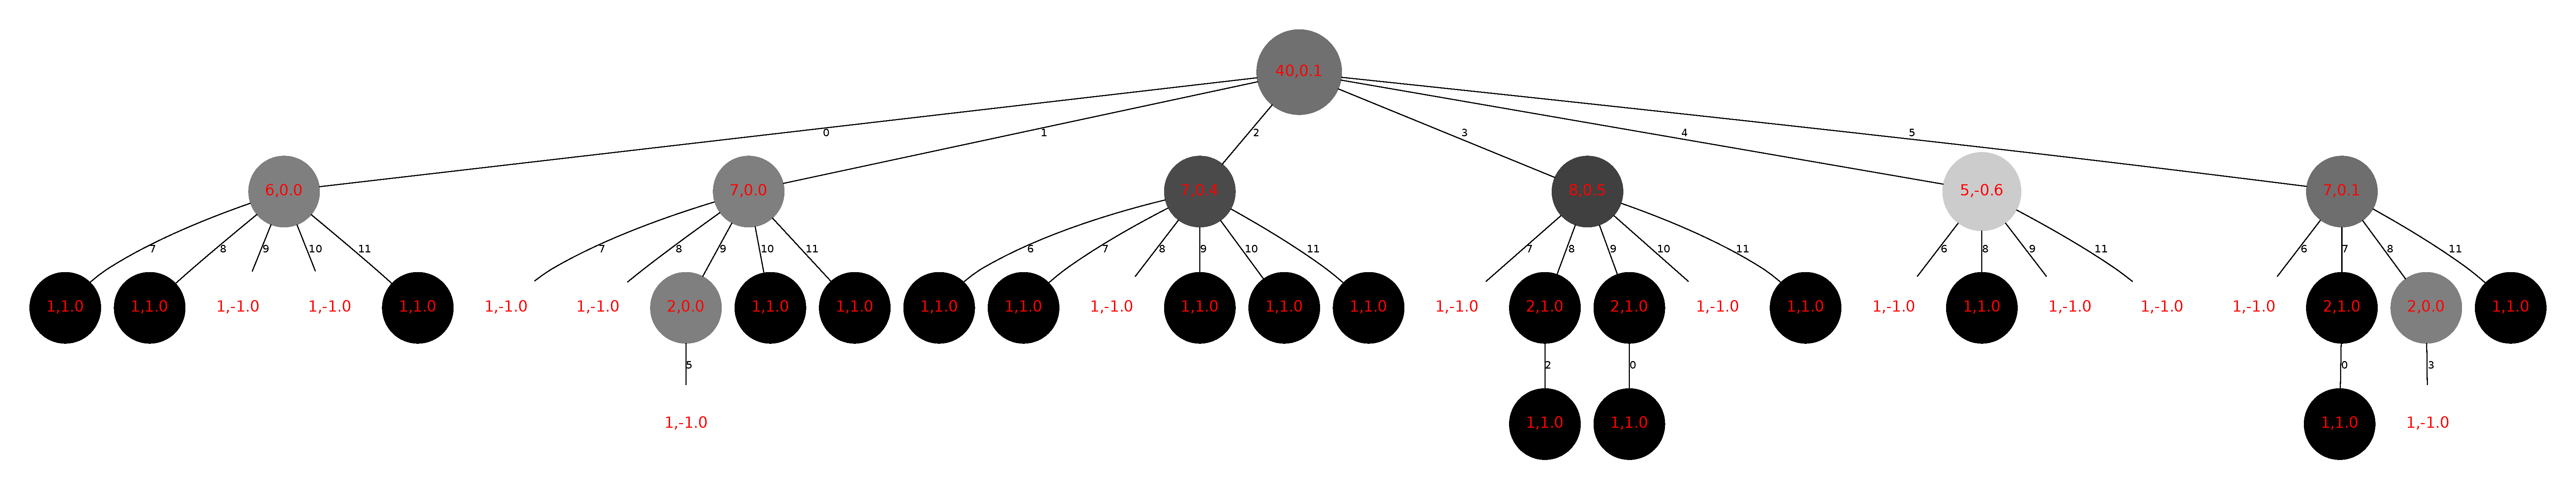
\includegraphics[width=\linewidth]{ressources/arbre_40_mcts.pdf}
    \caption{Un arbre de recherche pour la recherche arborescente de Monte Carlo}
  \end{figure}
\end{frame}

\begin{frame}
  \frametitle{Résultats de la recherche arborescente de Monte Carlo}
  \begin{figure}
    \centering
    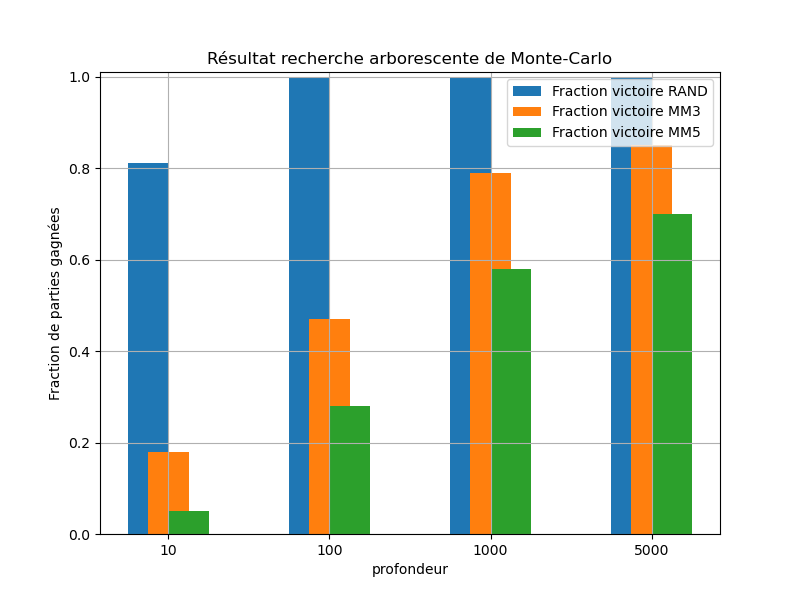
\includegraphics[width=0.7\linewidth]{ressources/resultat_mcts.png}
    \caption{Résultats de la recherche arborescente de Monte Carlo}
  \end{figure}
\end{frame}

\begin{frame}
  \frametitle{Un nouveau paradigme : l'analyse rétrograde}
  \begin{itemize}
  \item Utilisation de la programmation dynamique
  \end{itemize}
  \begin{block}{Anti-coups}
    Étant donné une configuration à $n$ pierres $A$, on dit que $A'$ est obtenue par anti-coup depuis la configuration $A$ si il existe un coup jouable dans $A'$ menant à la configuration $A$ sans récolte
  \end{block}
\end{frame}

\begin{frame}
  \frametitle{Explication de l'analyse rétrograde}
  L'algorithme se déroule en 3 étapes :
  \begin{itemize}
  \item Initialisation
  \item Convergence
  \item Stabilisation
  \end{itemize}
  Mais comment stocker toutes ses positions ?
\end{frame}

\begin{frame}
  \frametitle{Codage de Gödel}
  \begin{block}{Vecteur $\vec c$}
    Étant donné une configuration $A$, on note $A(i)$ le nombre de pierre dans le puit $i$. On pose $\vec c = (c_0, ..., c_{11})$ où $c_0 = A(0)$ et $c_{k+1}=A(k+1) + 1 + c_k$
  \end{block}
  \begin{block}{Codage de Gödel }
    On note, $$enc(\vec c) = \sum_{i=1}^{12} \binom {c_{i-1}} {i}$$
    Et on appelle nombre de Gödel de $A$ la quantité
    $$\mathcal E(A) = n + 25 \times enc(\vec c)$$ où $n$ est le nombre de pierres de $A$
  \end{block}
  Base de donnée construite pour $n = 29$
\end{frame}

\begin{frame}
  \frametitle{Conclusion}
\end{frame}

\begin{frame}
  \frametitle{Annexe 1 : Nombre d'états possible}
  Comment disposer $n$ objets indiscernables dans $k$ bacs (indexés) ?
  \begin{block}{La méthode des étoiles et des barres}
    Cela revient à dénombrer le nombre de manière de choisir $k-1$ barres pour séparer $n$ étoiles. Un bac pouvant être vide, tout arrangement d'étoiles et de barres se compose d'un total de $n + k - 1$ objets, dont $n$ étoiles et $k-1$ barres. On choisit donc $k-1$ barres parmi les $n+k-1$ positions possible.
    \begin{figure}
      \centering
      \caption{Une façon de partionner $8$ étoiles dans $5$ puits.}
      \includesvg[width=0.5\linewidth]{ressources/diagramme_stars_and_bars.svg}
    \end{figure}
    
  \end{block}

  Il y a donc $\binom {48+12-1}{12-1} = 279\ 871\ 768\ 995$ plateaux possibles.
\end{frame}
  

\end{document}

%%% Local Variables:
%%% mode: LaTeX
%%% TeX-master: t
%%% End:
